\section{\scshape Best views estimation}
\subsection*{Best views estimation}

\begin{frame}{Reference surface point cloud}
	\begin{itemize}
		\item The first step in the processing pipeline includes the generation of the multi-object reference point cloud that is assembled using the CAD data and the objects poses given by the simulator, which is later on filtered with a voxel grid algorithm to perform a regular spatial partition and extract the points that are in the surface voxels centroids
	\end{itemize}
	\begin{figure}
		\centering
		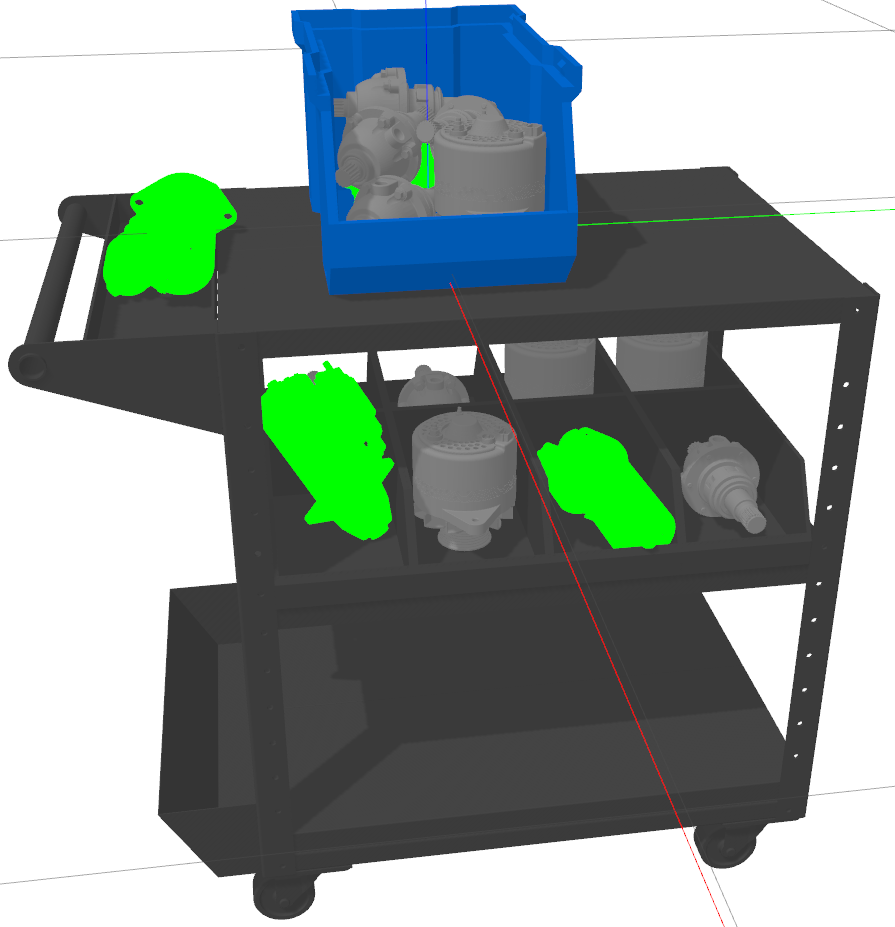
\includegraphics[height=.27\textheight]{sensor-data-processing/multimodel-environment}
		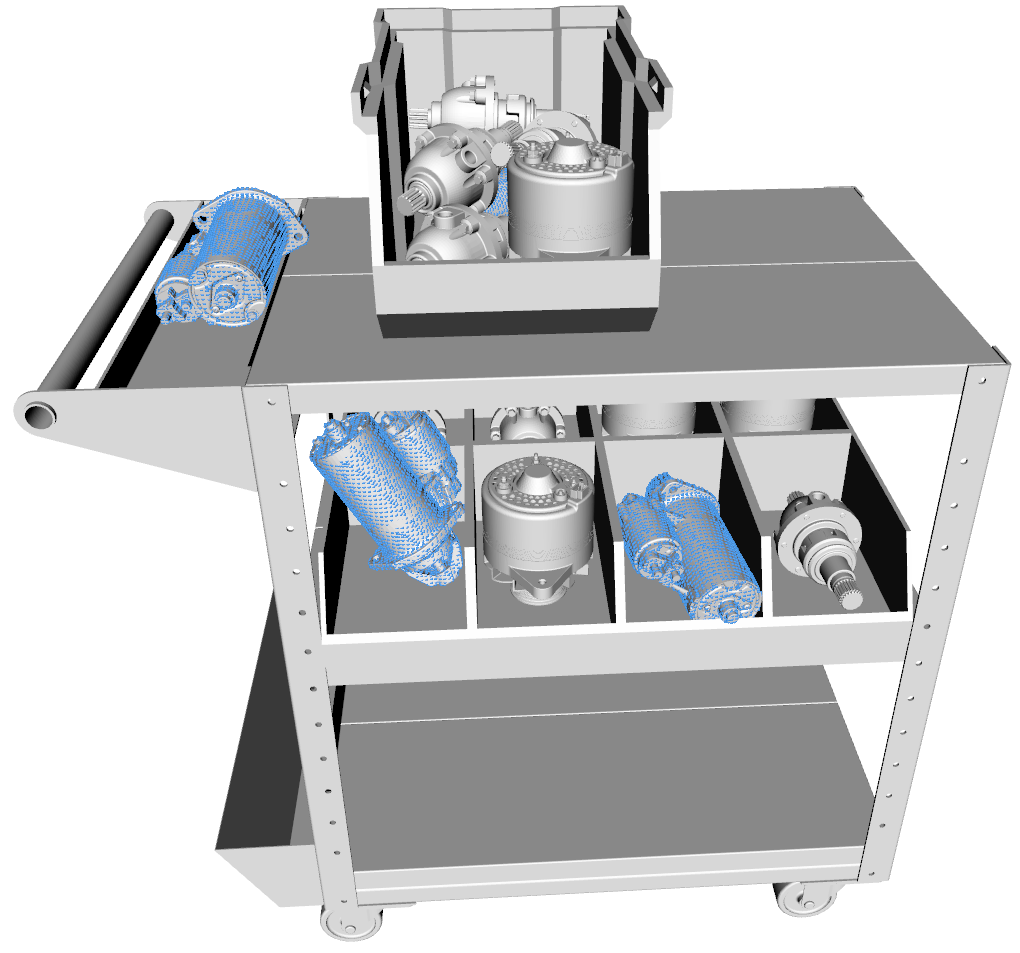
\includegraphics[height=.27\textheight]{sensor-data-processing/multimodel-pointclouds-with-cad}
		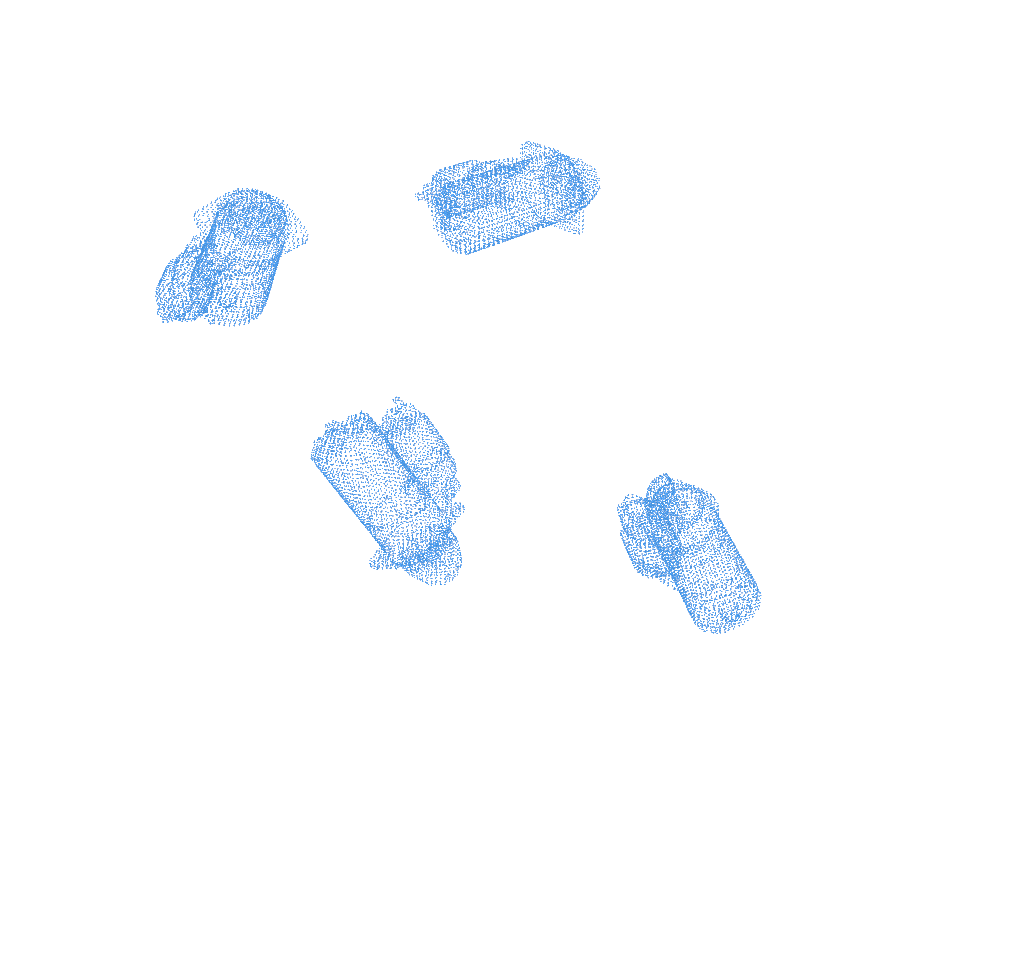
\includegraphics[height=.27\textheight]{sensor-data-processing/multimodel-pointclouds}
		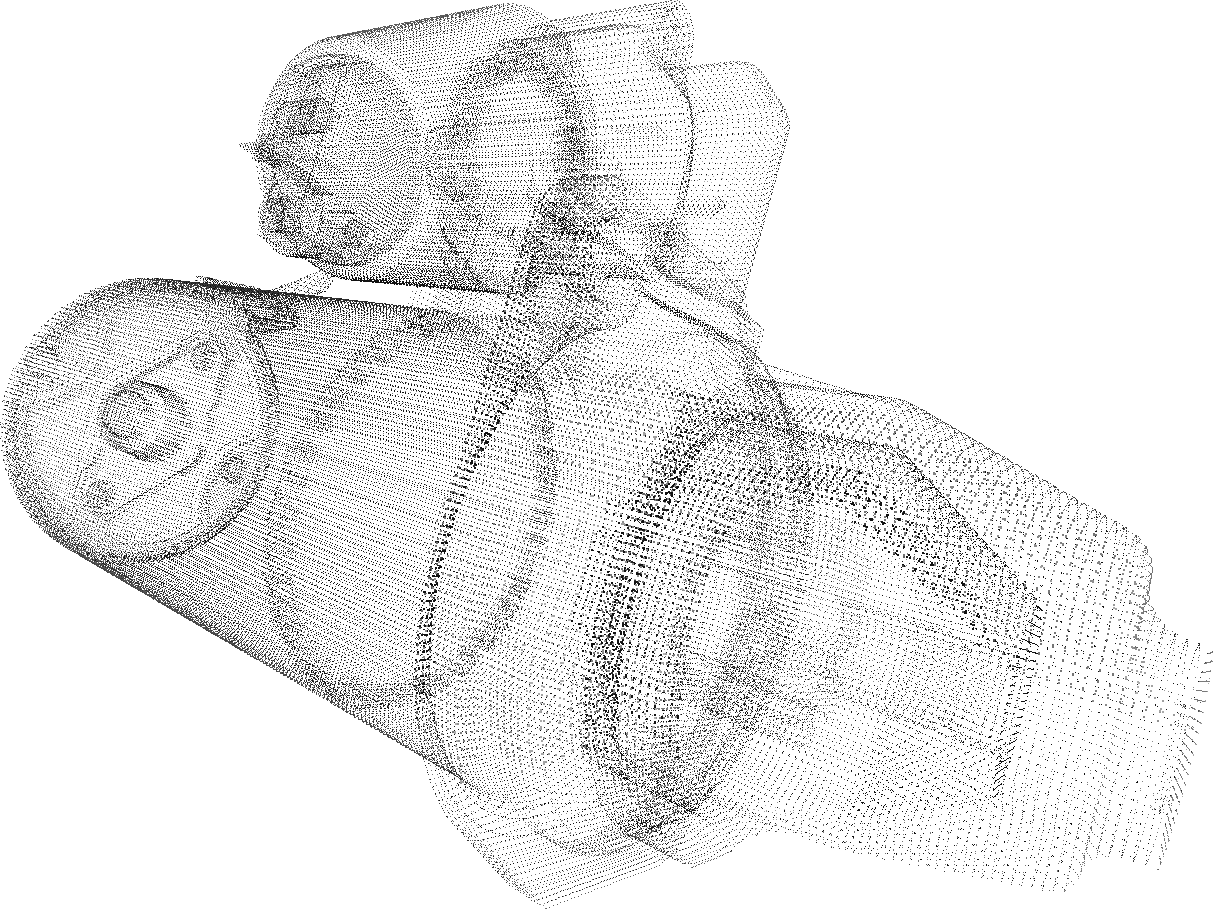
\includegraphics[height=.27\textheight]{sensor-data-processing/cad-model-pointcloud}
		\caption{The first image illustrates the color scene rendering in gazebo with the target objects in green while the second and third images display the reference point cloud that was generated from the CAD points data shown on the last image}
	\end{figure}
\end{frame}

\begin{frame}{Sensors data analysis}
	\begin{itemize}
		\item Given a set of deployed sensors in the simulation world, for each sensor it is computed the voxelized point cloud of the observed target object(s) points:
		\begin{itemize}
			\item Color segmentation is performed to identify the sensor image pixels that belong to the target object(s) (which have a unique pure green material)
			\item For the selected pixels, the depth points are generated using the pin hole camera model
			\item The generated point cloud is transformed from the sensor into the world coordinate system frame
			\begin{itemize}
				\item Allows fast merging of point clouds generated from different sensors
			\end{itemize}
			\item A voxel grid filtering algorithm is applied to perform a regular space partition in which the points centroid are computed for each voxel
			\begin{itemize}
				\item Critical for allowing consistent evaluation of the object(s) observed surface percentage, even when the sensors have different resolution and are at different distances from the target object(s)
			\end{itemize}
		\end{itemize}
	\end{itemize}
\end{frame}


\begin{frame}{Sensor data analysis}
	\begin{figure}
		\centering
		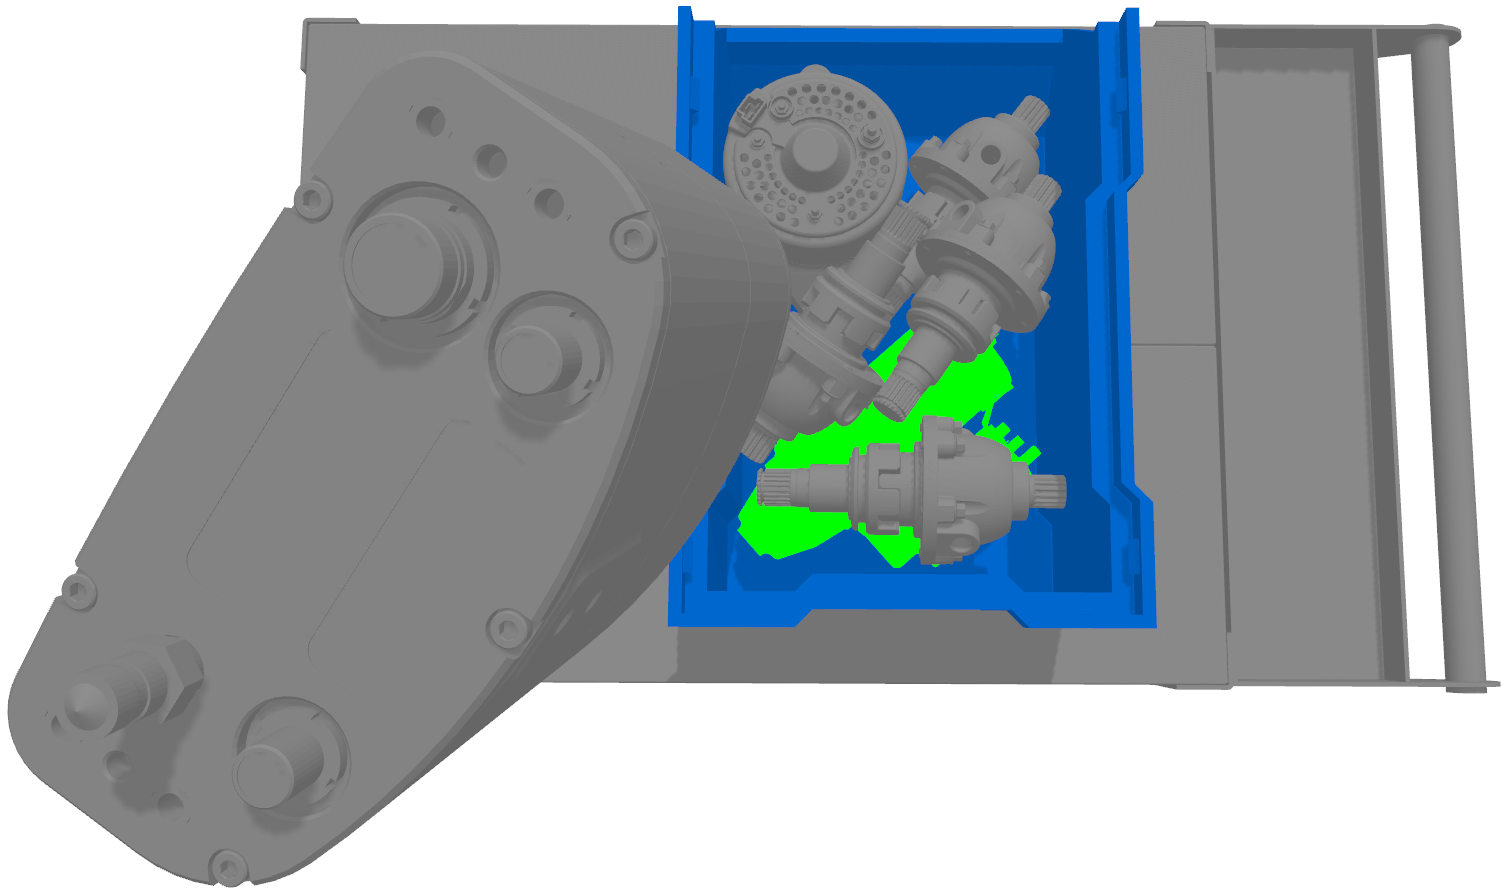
\includegraphics[height=.32\textheight]{sensor-data-processing/sensors-best-view}\\
		\vspace{0.5em}
		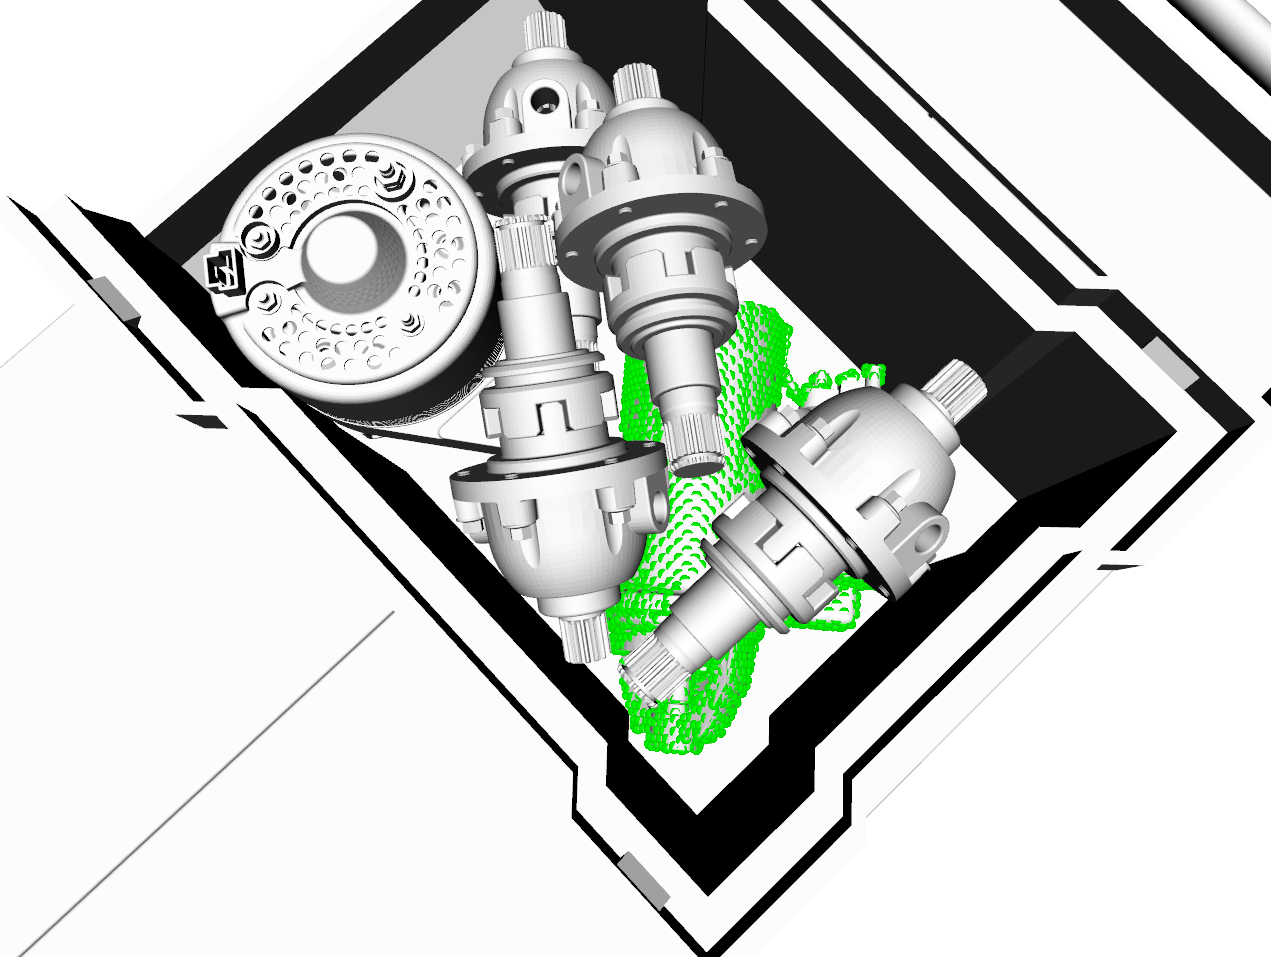
\includegraphics[height=.32\textheight]{sensor-data-processing/rviz-sensor-view}
		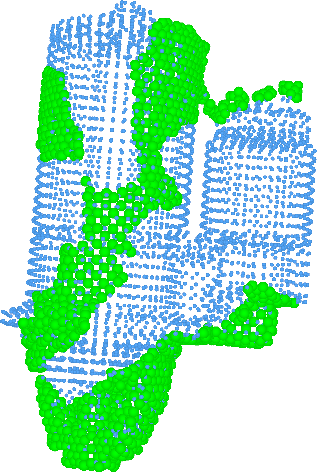
\includegraphics[height=.32\textheight]{sensor-data-processing/rviz-sensor-view-without-cad-with-model}
		\caption{Color image rendered with the gazebo simulator (top image containing the scene and sensor) along with the generated point cloud for the target object taking into consideration the environment occlusions (bottom images, in which the green spheres are the observed points and the blue spheres are from the point cloud of the associated CAD model)}
	\end{figure}
\end{frame}


\begin{frame}{Estimation of the best sensor configuration}
	After having the processed data for each deployed sensor:
	\begin{itemize}
		\item If only one sensor is enough:
		\begin{itemize}
			\item Compute the surface area percentage for each sensor
			\begin{itemize}
				\item Given that both the reference point cloud and sensor data were filtered with a voxel grid with the same resolution and in the same coordinate system frame, computing the surface percentage can be efficiently computed by simply dividing the number of surface voxel points in the sensor data by the number of surface voxel points in the reference point cloud
			\end{itemize}
			\item Choose the sensor that can observe the most surface area percentage of the object(s)
		\end{itemize}
	\end{itemize}
\end{frame}


\begin{frame}{Estimation of the best sensor configuration}
	After having the processed data for each deployed sensor:
	\begin{itemize}
		\item If several sensors can be used:
		\begin{itemize}
			\item Using a RANSAC approach, choose randomly a set of N sensors
			\item Merge the sensor data from the selected sensors
			\item Reapply the voxel filter algorithm to ensure that there are only one point per voxel
			\item Estimate the observable surface area percentage for the selected sensors
			\item If current subset of sensors achieved better observable surface percentage, then it becomes the current best views estimation for the sensor configuration
			\item At the end of a given number of iterations or if the observable surface percentage area reaches a given threshold, the search is terminated, keeping the best sensor configuration found
		\end{itemize}
	\end{itemize}
\end{frame}
